\chapter{Algorithms}\label{chap:algorithms}
This thesis examines three load balancing algorithms. First, the classic Push-Pull Sum algorithm and the Continuous Single-Proposal Deal-Agreement-Based algorithm are introduced. Next, the proposed Adaptive Threshold Push-Pull Sum algorithm is presented as a novel approach. The composition of this new algorithm is explained, including how it integrates elements of the first two algorithms and the rationale behind its design. For each algorithm, pseudo-code and a detailed description of their operational mechanics are provided. Additionally, examples are included to illustrate how the algorithms achieve load balancing. For the Adaptive Threshold Push-Pull Sum algorithm, the intended outcomes are also outlined to provide further clarity on its objectives.

\section{Characteristics}\label{sec:algoCharacteristics}
Like the graphs, load balancing algorithms may have different characteristics. In the following these characteristics are elaborated on:
\begin{itemize}
    \item \textbf{Static and Dynamic}: Load balancing algorithms can be categorized into static and dynamic algorithms. Static load balancing algorithms assign the tasks to the nodes at compile time. Dynamic load balancing algorithms assign the tasks at run-time. The main advantage that static load balancing algorithms have over dynamic load balancing algorithms is that they do not cause any run-time overhead \cite{Bokhari}.
    \item \textbf{Stochastic and Deterministic}: Stochastic load balancing algorithms use randomness in order to choose a load transfer partner. Deterministic load balancing algorithms on the other hand, use some predefined distribution rules in order to make load transfers. \cite{ChengzhongFrancis}
    \item \textbf{Global and Local}: For local load balancing algorithms nodes may only transfer loads within their domain/neighborhood, while a global load balancing algorithm enables the nodes in the network to perform load balancing operations across the whole network \cite{ChengzhongFrancis}. 
    \item \textbf{Monotonic and Non-monotonic}: A load balancing algorithm is characterized as monotonic, if each load transfer is from a higher loaded node to a less loaded node and the maximal load in the network never increases and the minimal load never decreases \cite{Dinitz2023DAB}.
    \item \textbf{Mass conservation property}: Load balancing algorithms may posses the mass conservation property, which ensures that the values will converge to the correct aggregate of the ground truth \cite{nugroho2023PushPullSumDataAg}.
    \item \textbf{Anytime}: An \textit{anytime} load balancing algorithm can be stopped at any time during the execution, and after stopage the state of the network is not worse than one of its preceding states. The advantage that comes with an anytime algorithm is that the network in which the load balancing algorithm with this property is applied to shows more feasible states with intermediate rounds. \cite{Dinitz2023DAB}
\end{itemize}
Many of these properties and characteristics are desirable for the load balancing algorithms to make the load balancing more efficient, like monotonicity or anytimeness. Others contribute to computational lightness like locality, and others guarantee predictability of the behaviour like determinism.

\section{Classic Push-Pull Sum Algorithm}\label{sec:classicPPS}
The Push-Pull Sum algorithm as proposed in \cite{nugroho2023PushPullSumDataAg} requires each node to have sum $s_{i,r}$ and weight $w_{i,r}$ values as initial information. The initial weight $w_{i,0}$ for each node is equal to 1. The sum of all weights is equal to the network size $N$. The sum of $s_{i,0}$ is equal to whatever the required input $x_i \in \mathbb{R}^{+}_{0}$ is, in the paper the values for the sums are uniformly distributed values between 0 and 100 \cite{nugroho2023PushPullSumDataAg}. The pseudo code is to be found in figure \ref{alg:PPS}. The Push-Pull Sum algorithm is composed of three different procedures, namely the \textit{RequestData} procedure, the \textit{ResponseData} procedure and the \textit{Aggregate} procedure. In every round $r$ the \textit{Aggregate} procedure is called, except for the first round, since there is no information to be aggregated. In this procedure, every node gatheres all incoming messages $M_{i,r}$ sent by other nodes $\{(s_m, w_m)\}$ in the previous round $r-1$, requesting data. Also, nodes update their sum values which essentially is $\sum_{m \in M_{i,r}}{s_m}$ and weight values $\sum_{m \in M_{i,r}}{w_m}$. The respective loads are calculated by dividing sum by weight. Following that, each node calls the \textit{RequestData} procedure. In this procedure, each node chooses a random neighbor node and executes a push operation, so each node sends half of its sum $\frac{s_{i,r}}{2}$ and half of its weight $\frac{w_{i,r}}{2}$ to the chosen node and itself. The pull mechanism is described in the \textit{ResponseData} procedure. Here, each node gathers the incoming requests per round $r$ in a set $R_{i, r}$. Then, each node replies to each requesting node (including itself) with the half of its sum value divided by the number of incoming requests, so $\frac{\frac{s_{i,r}}{2}}{|R_{i, r}|}$.

\renewcommand{\algorithmicrequire}{\textbf{Input:}}
\renewcommand{\algorithmicensure}{\textbf{Output:}}
\begin{algorithm}[]
\caption{Push-Pull Sum protocol}\label{alg:PPS}
\begin{algorithmic}[1]
\Procedure{RequestData}{}
\State Chose a random neighbor node $v$
\State Send $(\frac{s_{u,t}}{2}, \frac{w_{u,t}}{2})$ to the chosen node $v$ and the node $u$ itself
\EndProcedure
\Procedure{ResponseData}{}
\State $R_{u,t} \leftarrow$ Set of the nodes calling $u$ at a round $t$
\For{\textbf{all} $i \in R_{u,t}$}
\State Reply to i with $\left( \frac{\frac{s_{u,t}}{2}}{|R_{u,t}|}, \frac{\frac{w_{u,t}}{2}}{|R_{u,t}|} \right)$
\EndFor
\EndProcedure
\Procedure{Aggregate}{}
\State $M_{u,t} \leftarrow \{(s_{m}, w_{m})\}$ messages sent to $u$ at a round $t-1$
\State $s_{u,t} \leftarrow \sum_{m \in M_{u,t}}^{}s_{m}, w_{u,t} \leftarrow\sum_{m \in M_{u,t}}^{}w_{m}$
\State $f_{avg} \leftarrow \frac{s_{u,t}}{w_{u,t}}$
\EndProcedure
\end{algorithmic}
\end{algorithm}


The setting in the paper \cite{nugroho2023PushPullSumDataAg} is similar to ours. While they only inspect a complete graph with $10^{4}$ nodes, we have network sizes of $2^{10}$ nodes and more topologies under test. In that paper, 50 experiments each conducted for 30 rounds were performed. The paper showed that the Push-Pull Sum algorithm decreases the expected potential $\Phi_r$ exponentially. The potential function is defined as $\Phi_r=\sum_{i,j}\left(v_{i,j,r}-\frac{w_{i,r}}{n}\right)^{2}$. The $v_{i,j,r}$ component stores the fractional value of node $j$'s contribution at round $r$. The conditional expectation of $\Phi_r+1$ for the Push-Pull Sum algorithm is $\mathbb{E}[\Phi_r+1|\Phi_r=\phi]=(\frac{2e-1}{4e}-\frac{1}{4n})\phi$. The Push-Pull Sum algorithm has the mass-conservation property. Due to the fact that the load balancing algorithm orders its nodes to choose a random neighbor the load balancing algorithm is characterized as a stochastic load balancing algorithm. \cite{nugroho2023PushPullSumDataAg}

The Push-Pull Sum algorithm performed very well for the Complete graph, the Ring of Cliques with large clique size and Lollipop graphs with large clique size, and the Star graph. For the Star graph the internal node acts as a distributor of the load. While every leaf chooses with 100\% possibility the internal node as a "random" neighbor the internal node is involved as a endpoint of $N-1$ external push operations, and redistributes the load via pull operations to the leaves, where the sum is $\frac{\frac{s_{i,r}}{2}}{N-1}$ and accordingly the weight is $\frac{\frac{w_{i,r}}{2}}{N-1}$. A different explanation applies for the Complete graph, the Ring of Cliques and the Lollipop graph, where the density of each node plays an crucial role. Nodes choose a random neighbor, since the dense graphs have many edges, randomly choosing a neighbor allows the algorithm to spread loads effectively without relying on a deterministic path, reducing the likelihood of bottlenecks or overloading a single node. That is the reason, why the Push-Pull Sum algorithm did not perform so well for the Torus Grid graph and the Ring graph compared to the Single-Proposal Deal-Agreement-Based algorithm, where the number of edges is limited to $4$ and $2$ respectively. For these topologies redundant communication may occur, since two nodes may push back and fourth, with the sum being $\frac{s_{i,r}}{2}$ and the weight being $\frac{w_{i,r}}{2}$ for the push and pull operations. The result of this action is that the load values interact in such way that one node $u$ adopts the state of another node $v$ during the round, thus $load_{r}(u)=load_{r-1}(v)$ and vice versa, as described in chapter \ref{chap:appendix}. $load_{r}(u)$ represents the load of node $u$ at round $r$.
\subsection{Example}\label{subsec:examplePPS}
\begin{figure}
    \centering
    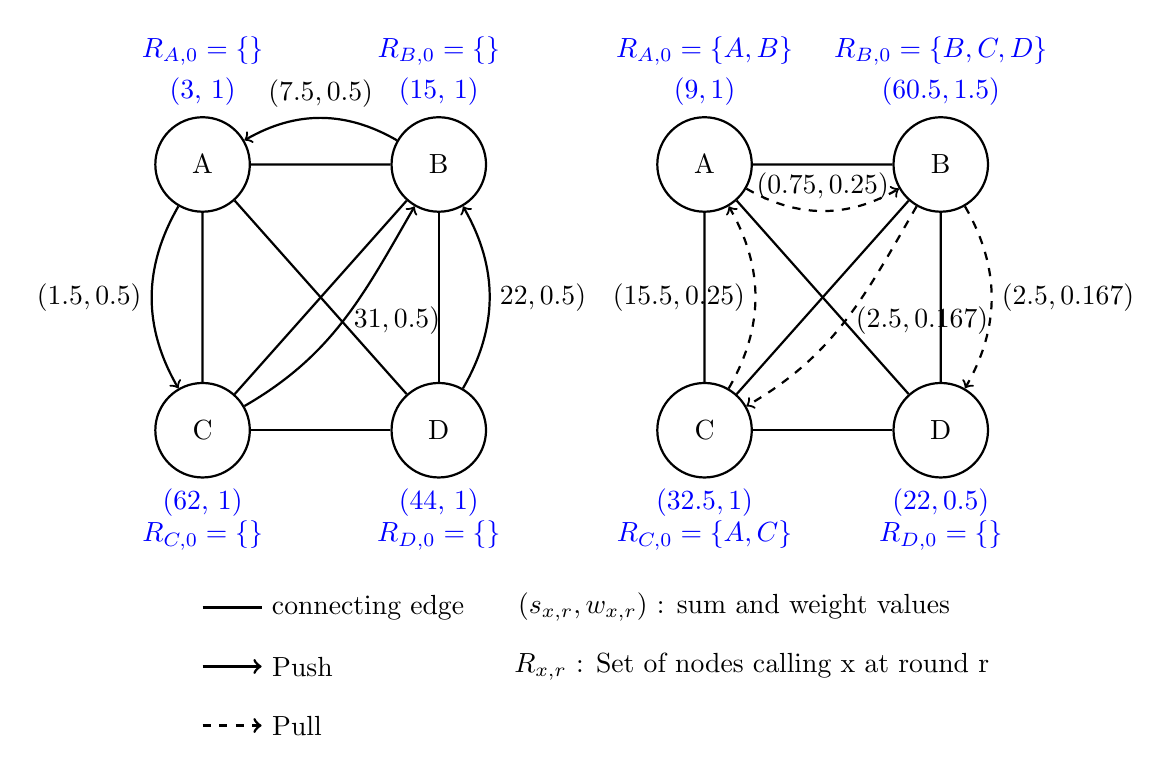
\begin{tikzpicture}[scale=0.75, thick, main node/.style={circle, draw, minimum size=1.2cm}]

    % First graph
    \node[main node] (A1) at (-1,4.5) {A};
    \node[main node] (B1) at (3,4.5) {B};
    \node[main node] (C1) at (-1,0) {C};
    \node[main node] (D1) at (3,0) {D};
    
    \node[above, color=blue] at (A1.north) {(3, 1)};
    \node[above, color=blue] at (B1.north) {(15, 1)};
    \node[below, color=blue] at (C1.south) {(62, 1)};
    \node[below, color=blue] at (D1.south) {(44, 1)};

    \node[above, color=blue] at (-1,6) {$R_{A,0}=\{\}$};
    \node[above, color=blue] at (3,6) {$R_{B,0}=\{\}$};
    \node[above, color=blue] at (-1,-2.2) {$R_{C,0}=\{\}$};
    \node[above, color=blue] at (3,-2.2) {$R_{D,0}=\{\}$};

     \node[above, color=blue] at (7.5,6) {$R_{A,0}=\{A, B\}$};
    \node[above, color=blue] at (11.5,6) {$R_{B,0}=\{B, C, D\}$};
    \node[above, color=blue] at (7.5,-2.2) {$R_{C,0}=\{A, C\}$};
    \node[above, color=blue] at (11.5,-2.2) {$R_{D,0}=\{\}$};
    
    \draw (A1) -- (B1);
    \draw (A1) -- (C1);
    \draw (A1) -- (D1);
    \draw (B1) -- (C1);
    \draw (B1) -- (D1);
    \draw (C1) -- (D1);

    % Second graph
    \node[main node] (A2) at (7.5,4.5) {A};
    \node[main node] (B2) at (11.5,4.5) {B};
    \node[main node] (C2) at (7.5,0) {C};
    \node[main node] (D2) at (11.5,0) {D};
    
    \node[above, color=blue] at (A2.north) {$(9, 1)$};
    \node[above, color=blue] at (B2.north) {$(60.5, 1.5)$};
    \node[below, color=blue] at (C2.south) {$(32.5, 1)$};
    \node[below, color=blue] at (D2.south) {$(22, 0.5)$};
    
    \draw (A2) -- (B2);
    \draw (A2) -- (C2);
    \draw (A2) -- (D2);
    \draw (B2) -- (C2);
    \draw (B2) -- (D2);
    \draw (C2) -- (D2);

    \draw[->] (A1) to[out=240, in=120] node[left] {$(1.5, 0.5)$} (C1);
    \draw[->] (B1) to[out=150, in=30] node[above] {$(7.5, 0.5)$} (A1);
    \draw[->] (C1) to[out=30, in=240] node[right] {$31, 0.5)$} (B1);
    \draw[->] (D1) to[out=60, in=300] node[right] {$22, 0.5)$} (B1);


    
    %\draw[dashed, ->] (C1) to[out=60, in=300] node[right] {$\frac{l_{C}-l_{A}}{2}$} (A1);
    %\draw[dashed, ->] (A1) to[out=330, in=210] node[right] {$\frac{l_{C}-l_{A}}{2}$} (B1);
    

    
    \draw[dashed, ->] (C2) to[out=60, in=300] node[left ] {$(15.5, 0.25)$} (A2);
     \draw[dashed, ->] (A2) to[out=-30, in=210] node[above] {$(0.75, 0.25)$} (B2);
     \draw[dashed, ->] (B2) to[out=240, in=30] node[right] {$(2.5,0.167)$} (C2);
          \draw[dashed, ->] (B2) to[out=300, in=60] node[right] {$(2.5,0.167)$} (D2);

    % Legend in the middle below the graphs
    \begin{scope}[shift={(3,-3)}]
        % Horizontal line
        \draw (-4,0) -- (-3,0) node[right] {connecting edge};
        % Long right arrow
        \draw[->, line width=1pt] (-4,-1) -- (-3,-1) node[right] {Push};
        % Long right dashed arrow
        \draw[->, dashed, line width=1pt] (-4,-2) -- (-3,-2) node[right] {Pull};
        
        % Load notation
        \node at (5,0) {$(s_{x,r}, w_{x,r})$ : sum and weight values};
        \node at (5.3,-1) {$R_{x,r}$ : Set of nodes calling x at round r};
    \end{scope}

\end{tikzpicture}
    \caption{Left: Push actions; Right: Pull actions}
    \label{fig:examplePPSSetting}
\end{figure}
The example in figure \ref{fig:examplePPSSetting} depicts a Complete graph $K_4$ (4 nodes) labeled from \textit{A} to \textit{D}. Each node has a initial sum and weight value assigned. The undirected graphs depict the connections between the nodes, indicating which nodes are neighboring nodes. The solid directed edges depict the push operations and the dashed directed edges depict the pull operations. Each node has a set $R_{i,r}$ where $i$ is the node id and $r$ is the round where we inspect the set. The load of the node is calculated by $\frac{s_{i,r}}{w_{i,r}}$. The example depicts the first round of a execution of the Push-Pull Sum algorithm. The push and pull operations are distinct. The left-hand side depicts the behaviour of the nodes while executing the push operations, while the right-hand side depicts the case of pull operations. Each node chooses a random neighbor to push load to. Node $A$ selected node $C$ and pushes half of its sum and weight to the chosen node $C$ and to itself (the loops are not included into the graphics, due to the readability of the figures). Node $B$ chose $A$ as a trading partner, node $C$ and $D$ push to node $B$ and themselves. Given the push operations for each node the set $R_{i,r}$ is computed. Due to node $B$ pushing load to node $A$ and node $A$ pushing load to itself, the set $R_{A,1}$ evaluates to $\{A,B\}$. The updated sum and weight values can be inspected on the right hand side of figure \ref{fig:examplePPSSetting}. Following the push actions, each node proceeds with the \textit{ResponseData}-procedure. For all the nodes in $R_{i,1}$ the nodes reply with the pull values. Since node $A$ has two nodes in its set $R_{A,1}$, node $A$ replies with $\left(\frac{\frac{3}{2}}{2}, \frac{\frac{1}{2}}{2}\right)$ to node $B$ and itself, indicated by a dashed directed edge. Accordingly, the remaining nodes \textit{B, C and D} execute the pull operations. Following the push and pull operations the nodes sum and weight values are updated. The setting after round one is depicted in figure \ref{fig:examplePPSResult}. The mean squared error in the beginning of round 1 is $542.50$, following one round of applying the Push-Pull Sum algorithm the mean squared error after round 1 is $63.49$.

\begin{figure}
    \centering
    \input{figures/Example_algos/PPS_Example_result.tex}
    \caption{Setting after round 1}
    \label{fig:examplePPSResult}
\end{figure}

\section{Contiunous Single-Proposal Deal-Agreement-Based Algorithm}\label{sec:singleproposalDAB}
The Continuous Single-Proposal Deal-Agreement-Based algorithm proposed by \cite{Dinitz2023DAB}, is unlike the Push-Pull Sum algorithm not an diffusion-based load balancing algorithm. The goal of load balancing is achieved based on deterministic deal-agreements, where one node proposes node to one neighboring node and the neighboring node either accepts the transfer proposal either full or partialy. Dinitz et al. proofed that the algorithm is a anytime algorithm, as they never worsen the state of the network during execution. They studied the algorithm in a dynamic setting. Each node has a set of neighboring nodes and their including the node's initial load itself as initial information. The algorithm is divided into three phases. There is the \textit{proposal}, \textit{deal} and the \textit{summary}-phase. In the \textit{proposal}-phase each node $u$ contacts the minimal loaded neighbor \textit{v} and sends a proposal to that neighbor, if the neighbor is less loaded. The proposal is of value $(\frac{load_{r}(u)-load_{r}(v)}{2})$, which is labeled as a \textit{fair} proposal. Since the load transfer is fair, the resulting load of $u$ is not lower than that of $v$. Following that, the nodes enter the \textit{deal}-phase. In this phase nodes evaluate the deals proposed to them. A node accepts the deal of the node that proposes the maximal load transfer. The actual transfer happens and the load values are being updated. Finally, in the \textit{summary}-phase each node informs their neighbors regarding their updated load values. \cite{Dinitz2023DAB}
\renewcommand{\algorithmicrequire}{\textbf{Input:}}
\renewcommand{\algorithmicensure}{\textbf{Output:}}
\begin{algorithm}
\caption{Continuous Single-Proposal Deal-Agreement-Based protocol}\label{alg:DAB}
\begin{algorithmic}[1]
\Require An undirected graph $G=(V,E,load)$
\Ensure A load state with discrepancy at most $\epsilon$ on $G$
\For{$r=1$ and on}
\For{every node u}
\State Find a neighbor, $v$, with the minimal load
\If{$load_{r}(u) - load_{r}(v)>0$}
\State $u$ sends to $v$ a transfer proposal of value $(load_{r}(u)-load_{r}(v))/2$
\EndIf
\EndFor

\For{every node $u$}
\If{there is at least one transfer proposal to $u$}
\State Find a neighbor, $w$, proposing to $u$ the maximal transfer
\State Node $u$ makes a deal: informs node $w$ on accepting its proposal
\State The actual transfer from $w$ to $u$ is executed 
\EndIf
\EndFor

\For{every node $u$}
\State Node $u$ sends the updated value of its load to its neighbors
\EndFor
\EndFor
\end{algorithmic}
\end{algorithm}


The analysis in this paper is based on a potential function. Dinitz et al. defines potential for a node $u$ as $p(u) = (load(u)-L_{avg})^{2}$ where $L_{avg}$ is the current load average in the network. The potential for the Graph $p(G)$ is defined as $p(G)=\sum_{u\in V}{p(u)}$, which essentially is the sum of all potential of each node in the graph G. Any fair load transfer of load $l$ decreases the potential of the graph by at least $2*l^{2}$. And as a result of any round $r$ of the Contiunous Single-Proposal Deal-Agreement-Based algorithm, the graph potential decreases by at least $\frac{K^{2}_r}{2D_r}$ where $K$ is the initial discrepancy and $D$ is a bound for the graph diameter. \cite{Dinitz2023DAB}

The Single-Proposal Deal-Agreement-Based load balancing algorithm seems to have difficulties in reducing the mean squared error as rapidly as the Push-Pull Sum algorithm for dense graphs like the a complete graph, the Lollipop graph with large clique size, the Ring of Cliques with large clique sizes. This seems to be the case, since each node is looking for a minimal load partner. For a Complete graph (and for the cliques respectively) the minimal load partner is the same node with loads of $L_{min}$. This causes each node to propose to the same node which then evaluates the proposals, and accepts exactly one transfer proposal, namely the maximal one. An analouge scenario happens for the Ring of Cliques and Lollipop graph, with the difference that for the Ring of Cliques not each node is proposing to the same minimal neighbor, but for the minimal laoded neighbor within their respective cliques. For the Lollipop graph, the nodes in the path graph balance their loads more quickly than the nodes in the clique which is a bottleneck in this scenario. Looking at the Torus Grid graph and the Ring graph, this Deal-Agreement-Based algorithm seems to perform very well in reducing the error, since the proposals are more distributed for the nodes due to the density of the graph, and thus more nodes are involved in load transfers. The Star graph makes an exception to this case, since we have a similar bottleneck as in the Complete graph, where the internal node is the common neighbor for each leaf and thus each leaf proposes load to the internal node. The internal node, then chooses only the maximal proposing transfer. The simulation results in the student project \cite{Bayazitoglu} indicate the performances of each load balancing algorithm for each topology very clearly.
\subsection{Example}\label{subsec:exampleDAB}
 \begin{figure}
    \centering
    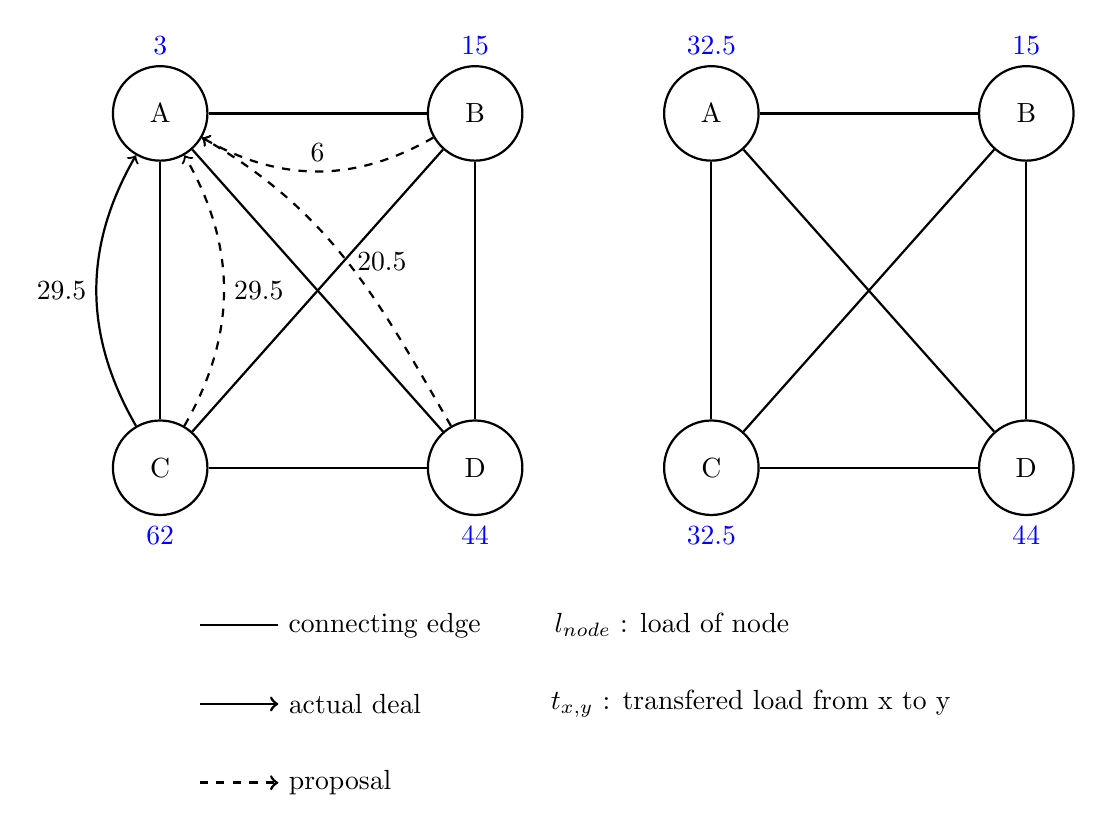
\begin{tikzpicture}[ thick, main node/.style={circle, draw, minimum size=1.2cm}]

    % First graph
    \node[main node] (A1) at (0.5,4.5) {A};
    \node[main node] (B1) at (4.5,4.5) {B};
    \node[main node] (C1) at (0.5,0) {C};
    \node[main node] (D1) at (4.5,0) {D};
    
    \node[above, color=blue] at (A1.north) {3};
    \node[above, color=blue] at (B1.north) {15};
    \node[below, color=blue] at (C1.south) {62};
    \node[below, color=blue] at (D1.south) {44};
    
    \draw (A1) -- (B1);
    \draw (A1) -- (C1);
    \draw (A1) -- (D1);
    \draw (B1) -- (C1);
    \draw (B1) -- (D1);
    \draw (C1) -- (D1);

    % Second graph
    \node[main node] (A2) at (7.5,4.5) {A};
    \node[main node] (B2) at (11.5,4.5) {B};
    \node[main node] (C2) at (7.5,0) {C};
    \node[main node] (D2) at (11.5,0) {D};
    
    \node[above, color=blue] at (A2.north) {32.5};
    \node[above, color=blue] at (B2.north) {15};
    \node[below, color=blue] at (C2.south) {32.5};
    \node[below, color=blue] at (D2.south) {44};
    
    \draw (A2) -- (B2);
    \draw (A2) -- (C2);
    \draw (A2) -- (D2);
    \draw (B2) -- (C2);
    \draw (B2) -- (D2);
    \draw (C2) -- (D2);

    \draw[->] (C1) to[out=120, in=240] node[left] {$29.5$} (A1);
    \draw[dashed, ->] (C1) to[out=60, in=300] node[right] {$29.5$} (A1);
    \draw[dashed, ->] (B1) to[out=210, in=330] node[above] {$6$} (A1);
    \draw[dashed, ->] (D1) to[out=120, in=330] node[right] {$20.5$} (A1);

    % Legend in the middle below the graphs
    \begin{scope}[shift={(3,-2)}]
        % Horizontal line
        \draw (-2,0) -- (-1,0) node[right] {connecting edge};
        % Long right arrow
        \draw[->, line width=1pt] (-2,-1) -- (-1,-1) node[right] {actual deal};
        % Long right dashed arrow
        \draw[->, dashed, line width=1pt] (-2,-2) -- (-1,-2) node[right] {proposal};
        
        % Load notation
        \node at (4,0) {$l_{node}$ : load of node};
        \node at (5,-1) {$t_{x,y}$ : transfered load from x to y};
    \end{scope}

\end{tikzpicture}
    \caption{Left: Initial Setup; Right: Result}
    \label{fig:DABExampleAlgo}
 \end{figure}
 Figure \ref{fig:DABExampleAlgo} depicts two settings. The setting is the same as in the example above in the Push-Pull Sum section, with the difference that each node has a load value assigned, instead sum and weight values. The dashed directed edge in this example represent a proposal from one node to another. The solid directed edge represents the actual load transfered from one node to another. We again consider the nodes \textit{A, B, C and D}. Each node looks for its minimal loaded neighbor. For nodes \textit{B, C and D} this is node $A$. For node $A$ this is node $B$, since node $B$ has more load than node $A$, node $A$ does not send an transfer proposal to node $B$. Nodes \textit{B, C and D} each send a transfer proposal of value $\frac{(load_r(i)-load_r(A))}{2}$ to node $A$, where $i \in \{B,C,D\}$. Node $A$ evaluates each transfer proposal and accepts node $C$'s transfer proposal, since node $C$ proposes the maximal amount of load, namely $29.5$. The actual transfer happens and $29.5$ of loads are transfered from node $C$ to node $A$. The right-hand side of figure \ref{fig:DABExampleAlgo} depicts the setting after round 1. Node $A$ and $C$ each have a load of $32.5$, the loads of nodes $B$
 and $D$ are unchanged. The mean squared in the beginning of round 1 is at $542.5$, in the end of round 1 the mean squared error decreases to a value of $107.375$, which is close to a fifth of the initial mean squared error. 

\section{Adaptive Threshold Push-Pull Sum Algorithm}\label{sec:adaptivethresholdPPS}
The Adaptive Threhsold Push-Pull Sum algorithm is composed of different ideas and elements of the two former algorithms, extended by the idea of adaptive thresholding. The Adaptive Threshold Push-Pull Sum consits of different procedures. In the \textit{CheckThresholdsRequestData} each node $i$ chooses a subset $RN$ of $\log_{2}{(|neighborhood|)}$ random neighbors. This is to enhance the chance of a good load transfer to happen. If we only choose one neighbor the chance is lower to find an optimal or good neighbor to execute a load transfer. Then the load difference between the node $i$ and each node in $RN$ is computed and checked if the load difference is bigger than some threshold $\theta$. The threshold is computed in the \textit{CalculateThresholds}-procedure. The threshold $\theta$ is computed as $k*\sqrt{MSE_r-1}$ where $k$ is some factor to adjust the sensitivity of the threshold. A larger $k$ means the threshold is more sensitive meaning that less nodes are eligiable for load transfer and respectively a lower $k$ means that the boundary is less strict, thus more nodes are eligiable for load transfer. This condition prevents load transfers with low effect, and guarantees a selection of nodes with effect above the given threshold. The first eligiable node receives the sum and the weight in form of a push action $(\frac{s_i,r}{2})$ for the sum and $(\frac{w_i,r}{2})$ for the weight. The \textit{ResponseData}, and the \textit{Aggregate}-procedure are analoge to the classic Push-Pull Sum algorithm. The push and the pull mechanism are directly taken from the Push-Pull Sum algorithm, and are combined with a adaptive threshold mechanism, thus the name Adaptive Threshold Push-Pull Sum algorithm. Two ideas are derived from the Single-Proposal Deal-Agreement-Based algorithm. The idea of the conditional load transfer is analog to the Single-Proposal Deal-Agreement-Based's one, with the only difference that the difference of load between the two negotiating nodes should not be larger than 0, but bigger than a threshold $\theta$. Furthermore, instead of initiaing a load transfer with the maximal loaded node, the Adaptive Threshold Push-Pull Sum algorithm orders the nodes to initiate a load transfer with the first node proposing load. The reason for that is to avoid that each node looks through the whole set $RN$ and needs to evaluate each proposal, instead the first node proposing a load transfer is accepted as a transfer partner.

Although not shown, the Adaptive Threshold Push-Pull Sum algorithm is expected to hold the mass conservation property, as it converged to the true ground truh for all the experiments, similiar to the Push-Pull Sum algorithm. One indication for this is that the push-pull mechanisms are adapted unchanged, and these operations are the only operations that let nodes transfer or receive node in the algorithm. Also the Adaptive Threhsold Push-Pull Sum algorithm is a stochastic algorithm as it chooses a subset of neighbors randomly.
\begin{algorithm}
    \caption{Adaptive Threshold Push-Pull Sum algorithm}\label{alg:PPS}
    \begin{algorithmic}[1]
    \Procedure{CalculateThresholds}{}
    \State $\theta \leftarrow k * \sqrt{MSE_{r-1}}$ 
    \EndProcedure
    \Procedure{CheckTresholdRequestData}{}
    \State $RN_{u,r} \leftarrow$ choose $\lceil \log_{2}{(|neighborhood(u)|)} \rceil$ random neighbor
    \For{every node $v_{i} \in RN_{u,r}$}
    \State $\Delta_{u, v_{i}} \leftarrow |(load_r(u) - load_r(v_{i}))|$
    \If{$\Delta_{u,v} > \theta$}
    \State Send $(\frac{s_{u,r}}{2}, \frac{w_{u,r}}{2})$ to first node v fulfilling condition and the node $u$ itself
    \EndIf
    \EndFor
    \EndProcedure
    \Procedure{ResponseData}{}
    \State $R_{u,r} \leftarrow$ Set of the nodes calling $u$ at a round $r$
    \For{\textbf{all} $i \in R_{u,r}$}
    \State Reply to i with $\left( \frac{\frac{s_{u,r}}{2}}{|R_{u,r}|}, \frac{\frac{w_{u,r}}{2}}{|R_{u,r}|} \right)$
    \EndFor
    \EndProcedure
    \Procedure{Aggregate}{}
    \State $M_{u,t} \leftarrow \{(s_{m}, w_{m})\}$ messages sent to $u$ at a round $r-1$
    \State $s_{u,t} \leftarrow \sum_{m \in M_{u,r}}^{}s_{m}, w_{u,r} \leftarrow\sum_{m \in M_{u,r}}^{}w_{m}$
    \State $load(u) \leftarrow \frac{s_{u,r}}{w_{u,r}}$
    \EndProcedure
    \end{algorithmic}
    \end{algorithm}
\subsection{Example}\label{subsec:exampleAdaptiveThresholdPPS}
\begin{figure}
    \centering
    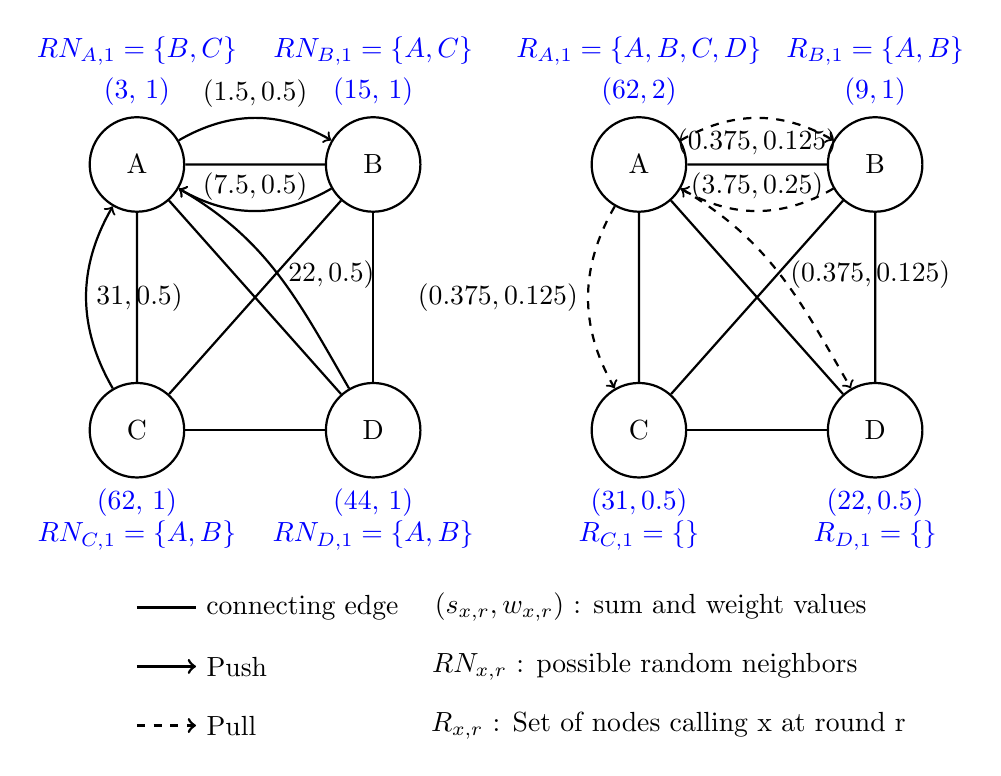
\begin{tikzpicture}[scale=0.75, thick, main node/.style={circle, draw, minimum size=1.2cm}]

    % First graph
    \node[main node] (A1) at (-1,4.5) {A};
    \node[main node] (B1) at (3,4.5) {B};
    \node[main node] (C1) at (-1,0) {C};
    \node[main node] (D1) at (3,0) {D};
    
    \node[above, color=blue] at (A1.north) {(3, 1)};
    \node[above, color=blue] at (B1.north) {(15, 1)};
    \node[below, color=blue] at (C1.south) {(62, 1)};
    \node[below, color=blue] at (D1.south) {(44, 1)};

    \node[above, color=blue] at (-1,6) {$RN_{A,1}=\{B,C\}$};
    \node[above, color=blue] at (3,6) {$RN_{B,1}=\{A,C\}$};
    \node[above, color=blue] at (-1,-2.2) {$RN_{C,1}=\{A,B\}$};
    \node[above, color=blue] at (3,-2.2) {$RN_{D,1}=\{A,B\}$};

     \node[above, color=blue] at (7.5,6) {$R_{A,1}=\{A, B, C, D\}$};
    \node[above, color=blue] at (11.5,6) {$R_{B,1}=\{A, B\}$};
    \node[above, color=blue] at (7.5,-2.2) {$R_{C,1}=\{\}$};
    \node[above, color=blue] at (11.5,-2.2) {$R_{D,1}=\{\}$};
    
    \draw (A1) -- (B1);
    \draw (A1) -- (C1);
    \draw (A1) -- (D1);
    \draw (B1) -- (C1);
    \draw (B1) -- (D1);
    \draw (C1) -- (D1);

    % Second graph
    \node[main node] (A2) at (7.5,4.5) {A};
    \node[main node] (B2) at (11.5,4.5) {B};
    \node[main node] (C2) at (7.5,0) {C};
    \node[main node] (D2) at (11.5,0) {D};
    
    \node[above, color=blue] at (A2.north) {$(62, 2)$};
    \node[above, color=blue] at (B2.north) {$(9, 1)$};
    \node[below, color=blue] at (C2.south) {$(31, 0.5)$};
    \node[below, color=blue] at (D2.south) {$(22, 0.5)$};
    
    \draw (A2) -- (B2);
    \draw (A2) -- (C2);
    \draw (A2) -- (D2);
    \draw (B2) -- (C2);
    \draw (B2) -- (D2);
    \draw (C2) -- (D2);

    \draw[->] (A1) to[out=30, in=150] node[above] {$(1.5, 0.5)$} (B1);
    \draw[->] (B1) to[out=210, in=-30] node[above] {$(7.5, 0.5)$} (A1);
    \draw[->] (C1) to[out=120, in=240] node[right] {$31, 0.5)$} (A1);
    \draw[->] (D1) to[out=120, in=-30] node[right] {$22, 0.5)$} (A1);


    
    %\draw[dashed, ->] (C1) to[out=60, in=300] node[right] {$\frac{l_{C}-l_{A}}{2}$} (A1);
    %\draw[dashed, ->] (A1) to[out=330, in=210] node[right] {$\frac{l_{C}-l_{A}}{2}$} (B1);
    

    
    \draw[dashed, ->] (A2) to[out=30, in=150] node[below] {$(0.375, 0.125)$} (B2);
     \draw[dashed, ->] (A2) to[out=240, in=120] node[left] {$(0.375, 0.125)$} (C2);
     \draw[dashed, ->] (A2) to[out=-30, in=120] node[right] {$(0.375,0.125)$} (D2);
      \draw[dashed, ->] (B2) to[out=210, in=-30] node[above] {$(3.75,0.25)$} (A2);

    % Legend in the middle below the graphs
    \begin{scope}[shift={(3,-3)}]
        % Horizontal line
        \draw (-4,0) -- (-3,0) node[right] {connecting edge};
        % Long right arrow
        \draw[->, line width=1pt] (-4,-1) -- (-3,-1) node[right] {Push};
        % Long right dashed arrow
        \draw[->, dashed, line width=1pt] (-4,-2) -- (-3,-2) node[right] {Pull};
        
        % Load notation
        \node at (4.7,0) {$(s_{x,r}, w_{x,r})$ : sum and weight values};
        \node at (4.6,-1) {$RN_{x,r}$ : possible random neighbors};
        \node at (5,-2) {$R_{x,r}$ : Set of nodes calling x at round r};
    \end{scope}

\end{tikzpicture}
    \caption{Left: Push actions; Right: Pull actions}
    \label{fig:ATPPSExampleSetting}
\end{figure}
Figure \ref{fig:ATPPSExampleSetting} depicts a similar setting as described in the section \ref{subsec:examplePPS}. Now, according to the Adaptive Threshold Push-Pull Sum algorithm, each node chooses $\log_{2}{(|neighborhood|)}$ neighbors. For this setting, this means that each node chooses 2 neighbors. These neighbors are added to the set $RN_{i,1}$ for each node $i$. For instance, node $A$ computed $RN_{A,1}$ as $\{B,C\}$. The load differences between node $A$ and nodes $B$ and $C$ are computed respectively. In this example, $k$ is $0.01$, thus the threshold $\theta$ in this case is $0.01*\sqrt{542.5} \approx 0.23$. Since both load differences between nodes $A$ and $B$, and nodes $A$ and $C$ pass this threshold, both nodes are eligiable to propose to transfer load with node $A$. In this scenario node $A$ chooses node $B$ as a transfer partner and pushes half of its sum $1.5$ and weight $0.5$ to node $B$ and itself. Accordingly, for each node respectively. Similar to the example in section \ref{subsec:examplePPS} the nodes execute the pull operation. The result is depicted in figure \ref{fig:ATPPSExampleResult}. The mean squared error dropped from $542.5$ initially, to $251.86$.
\begin{figure}
    \centering
    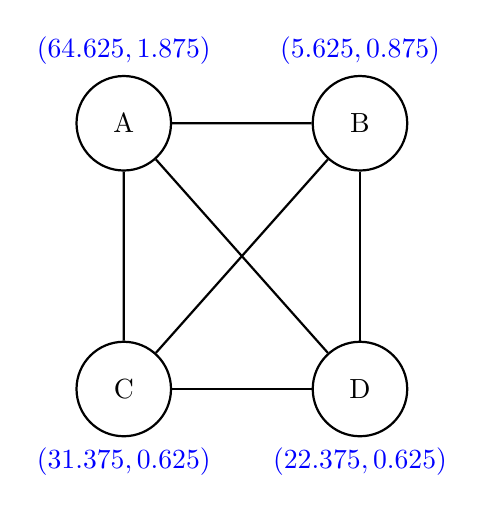
\begin{tikzpicture}[scale=0.75, thick, main node/.style={circle, draw, minimum size=1.2cm}]

    % First graph
    \node[main node] (A1) at (-1,4.5) {A};
    \node[main node] (B1) at (3,4.5) {B};
    \node[main node] (C1) at (-1,0) {C};
    \node[main node] (D1) at (3,0) {D};
    
    \node[above, color=blue] at (A1.north) {$(64.625,1.875)$};
    \node[above, color=blue] at (B1.north) {$(5.625, 0.875)$};
    \node[below, color=blue] at (C1.south) {$(31.375, 0.625)$};
    \node[below, color=blue] at (D1.south) {$(22.375, 0.625)$};
    
    \draw (A1) -- (B1);
    \draw (A1) -- (C1);
    \draw (A1) -- (D1);
    \draw (B1) -- (C1);
    \draw (B1) -- (D1);
    \draw (C1) -- (D1);

\end{tikzpicture}
    \caption{Setting after round 1}
    \label{fig:ATPPSExampleResult}
\end{figure}
\subsection{Aspired Outcome}\label{subsec:aspiredOutcomeAdaptiveThresholdPPS}
Thinking of the simulation results presented in \cite{Bayazitoglu} the discrepancy between the MSE reduction per round for the different topologies show that the algorithms perform either very well or medicore to bad. The main idea and perspective designing this algorithm was to find a compromise solution to that, to provide a better adaptability for different network topologies.

The final results of the first load balancing step can be taken from table \ref{tab:overviewExamples}. The Push-Pull Sum algorithm shows the lowest mean squared error after round 1, followed by the Deal-Agreement-Based algorithm and the Adaptive Threshold Push-Pull Sum algorithm. In section \ref{chap:simulationoutcomes} we will see that the Adaptive Threshold Push-Pull Sum algorithm proceeds to enhance in reducing error in later rounds, as the MSE and thus the threshold adjusts.
\begin{table}[]
\begin{tabular}{|c|c|c|c|c|}
\hline
 & \textbf{Initial} & \textbf{Dinitz et al.} & \textbf{Nugroho et al.} & \textbf{Bayazitoglu} \\ \hline
\textbf{Node A}  & 3      & 32.5    & (23.75, 1) = 23.75     & (64.625, 1.875) = 34.47 \\ \hline
\textbf{Node B}  & 15     & 15      & (56.25, 1.416) = 39.72 & (5.625, 0.875) = 6.43   \\ \hline
\textbf{Node C}  & 62     & 32.5    & (19.5, 0.9167) = 21.27 & (31.375, 0.625) = 50.2  \\ \hline
\textbf{Node D}  & 44     & 44      & (24.5, 0.67) = 36.57   & (22.375, 0.625) = 35.8  \\ \hline
\textbf{MSE} & 542.50 & 107.375 & 63.49                  & 251.86                  \\ \hline
\end{tabular}
\caption{Overview over example outcomes}
\label{tab:overviewExamples}
\end{table}